%! suppress = LineBreak
\documentclass[11pt, a4paper, hidelinks]{article}
\usepackage[utf8]{inputenc}
\usepackage{amsmath}
\usepackage{amsfonts}
\usepackage{amssymb}
\usepackage{amsthm}
\usepackage{graphicx}
\usepackage{hyperref}
\usepackage{geometry}
\geometry{a4paper, margin=0.5in}
\usepackage{fancyhdr}
\usepackage{indentfirst} % Add this line to enable first paragraph indentation
\usepackage{times} % Use Times New Roman font
\usepackage{setspace}
\usepackage[width=0.9\textwidth]{caption}
\usepackage{array}
\usepackage{float}
\usepackage{makecell}
\usepackage{longtable}

\setstretch{1.0} % Adjust the stretch factor as needed

\pagestyle{fancy}
\fancyhf{}  % Clear header and footer fields
\rfoot{\thepage}  % Place page number at the right bottom corner
\renewcommand{\headrulewidth}{0pt}  % Remove the header line

\begin{document}

% Title Page
\begin{titlepage}
    \centering
    \vspace*{0.5 cm}
    
\includegraphics[width=0.20\textwidth]{logo.png}\par\vspace{1cm}
    {\scshape\LARGE Warsaw University of Technology \par}
    \vspace{1cm}
    {\scshape\Large Faculty of Mathematics and Information Science\par}
    \vspace{1.5cm}
    {\huge\bfseries Project 3 Report\par}
    \vspace{1cm}
    {\Large\itshape Bioinformatics\par}
    \vfill
    % \vspace{2cm}
    \begin{flushright}

    {\Large\bfseries Nikita Kozlov (317099)\par}
    \vfill
    {supervisor\par}
    {\Large dr Michał Własnowolski \par}

    \end{flushright}
    \vfill
    % \break
    {\large Warsaw 2024\par}
    \vspace{1cm}
\end{titlepage}

\tableofcontents

\newpage

\section{Introduction}\label{sec:introduction}
\addcontentsline{}{section}{Introduction}

\subsection{Aim}\label{subsec:aim}

The aim of this project is to conduct a phylogenetic analysis of a set of protein sequences for a common set of species. The analysis will be based on the multiple sequence alignment of the sequences and the construction of a phylogenetic tree.

8 human proteins were selected for the analysis. For these proteins, through the use of BLAST, sequences were obtained for 7 species with the similarity to the human proteins not higher than 97\%.

Then, the sequences are aligned and clustered, and results are checked against the known taxonomy of the species.

\subsection{Data}\label{subsec:data}

Eight human proteins were selected for this analysis. For each protein, homologous sequences were obtained from different organisms using BLAST. Table~\ref{tab:proteins} lists the selected proteins and their general functions, while Table~\ref{tab:organisms} shows the organisms used in the analysis.

\begin{table}[H]
    \centering
    \caption{Selected proteins for phylogenetic analysis}
    \label{tab:proteins}
    \begin{tabular}{|p{0.3\textwidth}|p{0.6\textwidth}|}
        \hline
        \textbf{Identifier} & \textbf{Protein Name} \\
        \hline
        CAA84380.1 & Human histamine H1 receptor \\
        \hline
        NP\_001381685.1 & TANK-binding kinase 1-binding protein 1 \\
        \hline
        AAA59172.1 & Insulin \\
        \hline
        1PPF\_E & Human leukocyte elastase \\
        \hline
        AAA63214.1 & Melanin concentrating hormone \\
        \hline
        AAB03393.1 & Thrombopoietin \\
        \hline
        AAB50706.1 & Ficolin \\
        \hline
        NP\_570139.3 & Tetraspanin-18 \\
        \hline
    \end{tabular}
\end{table}

\begin{table}[H]
    \centering
    \caption{Organisms selected for comparative analysis}
    \label{tab:organisms}
    \begin{tabular}{|l|l|}
        \hline
        \textbf{Scientific Name} & \textbf{Common Name} \\
        \hline
        Pongo abelii & Sumatran orangutan \\
        Macaca fascicularis & Crab-eating macaque \\
        Cercocebus atys & Sooty mangabey \\
        Trachypithecus francoisi & François's langur \\
        Piliocolobus tephrosceles & Ugandan red colobus \\
        Eulemur rufifrons & Red-fronted lemur \\
        Macaca mulatta & Rhesus macaque \\
        Macaca nemestrina & Southern pig-tailed macaque \\
        \hline
    \end{tabular}
\end{table}

The sequences were selected to maintain sufficient evolutionary distance while ensuring reliable sequence alignment. All sequences show less than 97\% identity to their human homologs, allowing for meaningful phylogenetic analysis. The selected organisms represent different primate lineages, including Old World monkeys, New World monkeys, and prosimians, providing a broad evolutionary perspective for the analysis.

\section{Methodology}\label{sec:methodology}

\subsection{Methods and algorithms}\label{subsec:methods-and-algorithms}

The analysis was conducted using several bioinformatics tools and algorithms:

\paragraph{Sequence Analysis Tools}
\begin{itemize}
    \item BLAST (Basic Local Alignment Search Tool) for identifying homologous sequences
    \item MUSCLE (MUltiple Sequence Comparison by Log-Expectation) for multiple sequence alignment
    \item CD-HIT for sequence clustering with 50\% identity threshold
\end{itemize}

\paragraph{Programming Libraries}
\begin{itemize}
    \item BioPython for sequence manipulation and phylogenetic analysis
    \item Bio.Phylo for tree construction and visualization
    \item Bio.AlignIO for handling multiple sequence alignments
    \item Bio.SeqIO for sequence file parsing
\end{itemize}

\paragraph{Distance Calculations}
\begin{itemize}
    \item Identity-based distance matrix calculation using BioPython's DistanceCalculator
    \item Pairwise sequence comparison for evolutionary distance estimation
\end{itemize}

\paragraph{Visualization Tools}
\begin{itemize}
    \item Matplotlib for tree visualization and plotting
    \item BioPython's tree drawing functions for phylogenetic tree representation
\end{itemize}

All analyses were performed using Python 3, with custom scripts for data processing and visualization. The complete analysis pipeline was automated to ensure reproducibility of results.

\subsection{Selection of Common Organisms}\label{subsec:selection-of-common-organisms}

The selection of organisms for comparative analysis was performed using an automated algorithm to ensure consistency across all protein groups. The process involves several steps:

\noindent First, reference sequences for each human protein were collected and parsed using BioPython's SeqIO module.

\noindent For each protein, BLAST results were analyzed to identify homologous sequences from different organisms. The algorithm processes these raw sequences using the following steps:

\begin{itemize}
    \item Parse all BLAST result files, extracting metadata including organism names and sequence identifiers
    \item Count the frequency of each organism's appearance across all BLAST results
    \item Sort organisms by their frequency of occurrence
    \item Select the top 7 most common organisms that have homologs for most proteins
\end{itemize}

\noindent For each protein group, the algorithm then:
\begin{itemize}
    \item Takes the human reference sequence
    \item Selects homologous sequences from the identified common organisms
    \item Ensures no duplicate organisms are included
    \item Creates a final set of exactly 8 sequences (1 human + 7 homologs)
\end{itemize}

\noindent This approach ensures that:
\begin{itemize}
    \item Each protein group has the same set of organisms
    \item The selected organisms have good coverage across all proteins
    \item The selection process is systematic and reproducible
\end{itemize}

\noindent The organisms were selected based on their representation in BLAST results, resulting in a set of closely related primate species that allows for meaningful evolutionary comparison.

\subsection{Analysis steps}\label{subsec:analysis-steps}


The analysis was conducted through several sequential computational steps:

\paragraph{Multiple Sequence Alignment (MSA)}
All sequences were first merged into a single FASTA file for comprehensive analysis. The MUSCLE algorithm was used to perform multiple sequence alignment on the entire dataset. This approach ensures that:
\begin{itemize}
    \item All sequences are aligned consistently
    \item Homologous positions across different proteins are identified
    \item Gaps are introduced appropriately to maximize alignment quality
\end{itemize}

\paragraph{Distance Matrix Construction}
Following the MSA, a distance matrix was constructed using the following steps:
\begin{itemize}
    \item The aligned sequences were processed using BioPython's AlignIO module
    \item Pairwise distances were calculated using the 'identity' metric
    \item The resulting distance matrix captures the evolutionary relationships between all sequences
\end{itemize}

\paragraph{Sequence Clustering}
CD-HIT was employed for sequence clustering with the following parameters:
\begin{itemize}
    \item Sequence identity threshold (-c): 0.5
    \item Word length (-n): 2
\end{itemize}

The clustering analysis revealed 8 distinct clusters, which showed strong correspondence with the original protein groups:
\begin{itemize}
    \item Cluster 0: TANK-binding kinase 1-binding protein 1
    \item Cluster 1: Thrombopoietin
    \item Cluster 2: Histamine H1 receptor
    \item Cluster 3: Ficolin
    \item Cluster 4: Human leukocyte elastase
    \item Cluster 5: Tetraspanin-18
    \item Cluster 6: Melanin concentrating hormone
    \item Cluster 7: Insulin
\end{itemize}

This clustering result validates our initial protein selection, confirming that each group represents a distinct protein family with well-preserved sequence characteristics across different organisms.

\paragraph{Tree Construction}
Using the distance matrix, three different approaches to phylogenetic tree construction were implemented:

\begin{enumerate}
    \item \textbf{Individual Protein Trees:}
    \begin{itemize}
        \item Separate phylogenetic trees were constructed for each of the 8 protein groups
        \item Each tree contained sequences from all selected organisms for that specific protein
        \item UPGMA algorithm was used for tree construction
    \end{itemize}

    \item \textbf{Cluster-based Trees:}
    \begin{itemize}
        \item Separate trees were constructed for each CD-HIT cluster
        \item This approach grouped sequences based on similarity rather than initial protein classification
    \end{itemize}

    \item \textbf{Comprehensive Tree:}
    \begin{itemize}
        \item A single large phylogenetic tree was constructed using all sequences
        \item This tree provides a global view of relationships between all proteins and organisms
    \end{itemize}
\end{enumerate}

\paragraph{Consensus Trees}
Two types of consensus trees were generated to compare different classification approaches:
\begin{itemize}
    \item A majority consensus tree from all individual protein trees
    \item A majority consensus tree from all cluster-based trees
\end{itemize}

\paragraph{Visualization}
The trees were visualized with two different coloring schemes for comparative analysis:
\begin{itemize}
    \item Organism-based coloring: branches colored according to the source organism
    \item Protein-based coloring: branches colored according to the protein group
\end{itemize}

\noindent This dual coloring approach allows for visual analysis of both evolutionary relationships between organisms and functional relationships between proteins.

\noindent This clustering result validates our initial protein selection, confirming that each group represents a distinct protein family with well-preserved sequence characteristics across different organisms.

\section{Results}\label{sec:random-sequence-generation}

\subsection{Comparison of Protein Groups and Clusters}\label{subsec:comparison-of-protein-groups-and-clusters}

The analysis revealed strong correspondence between the original protein groups and the clusters obtained through CD-HIT analysis. Figure \ref{fig:tree_comparison} shows the matching between original protein groups and their corresponding clusters:

\begin{figure}[H]
    \centering
    \begin{tabular}{|l|l|l|}
        \hline
        \textbf{Original Group} & \textbf{Protein Name} & \textbf{Corresponding Cluster} \\
        \hline
        1PPF\_E & Human leukocyte elastase & Cluster 4 \\
        NP\_570139 & Tetraspanin-18 & Cluster 5 \\
        CAA84380 & Histamine H1 receptor & Cluster 2 \\
        AAB50706 & Ficolin & Cluster 3 \\
        AAB03393 & Thrombopoietin & Cluster 1 \\
        AAA63214 & Melanin concentrating hormone & Cluster 6 \\
        AAA59172 & Insulin & Cluster 7 \\
        NP\_001381685 & TANK-binding kinase 1-binding protein 1 & Cluster 0 \\
        \hline
    \end{tabular}
    \caption{Correspondence between original protein groups and CD-HIT clusters}
    \label{fig:tree_comparison}
\end{figure}

Comparing the phylogenetic trees of corresponding groups and clusters reveals several interesting patterns:

\begin{enumerate}
    \item The topological structure of trees is highly conserved between original groups and their corresponding clusters. For example, the trees for Histamine H1 receptor (CAA84380) and Cluster 2 show identical branching patterns and similar branch lengths.

    \item
        Both approaches consistently group closely related species together:
        \begin{itemize}
            \item Macaca species (M. fascicularis, M. nemestrina, M. mulatta) consistently form tight clusters
            \item Human (Homo sapiens) and Orangutan (Pongo abelii) are typically placed as sister groups
            \item Old World monkeys (Cercocebus, Trachypithecus, Piliocolobus) form distinct clades
        \end{itemize}

    \item The branch lengths, representing evolutionary distances, are remarkably similar between corresponding trees, suggesting that both approaches capture similar evolutionary relationships.

    \item Some differences are observed in the placement of more distant species like Eulemur rufifrons, particularly in proteins that show higher evolutionary rates.
\end{enumerate}

\subsection{Comparison of Individual Trees}\label{subsec:comparison-of-individual-trees}

\begin{longtable}{|c|c|}
%    \begin{tabular}
        \hline
        \textbf{Original Protein Tree} & \textbf{Corresponding Cluster Tree} \\
        \hline
        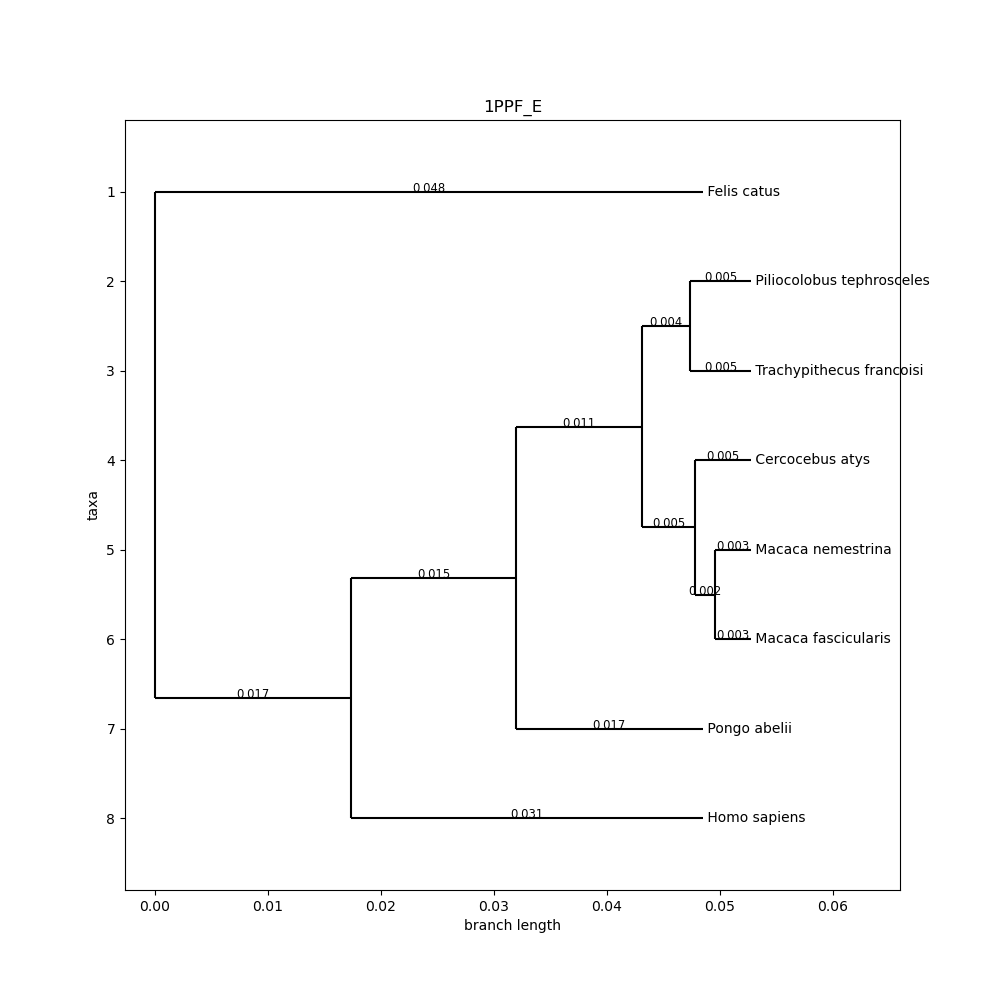
\includegraphics[width=0.45\textwidth]{1PPF_E.png} &
        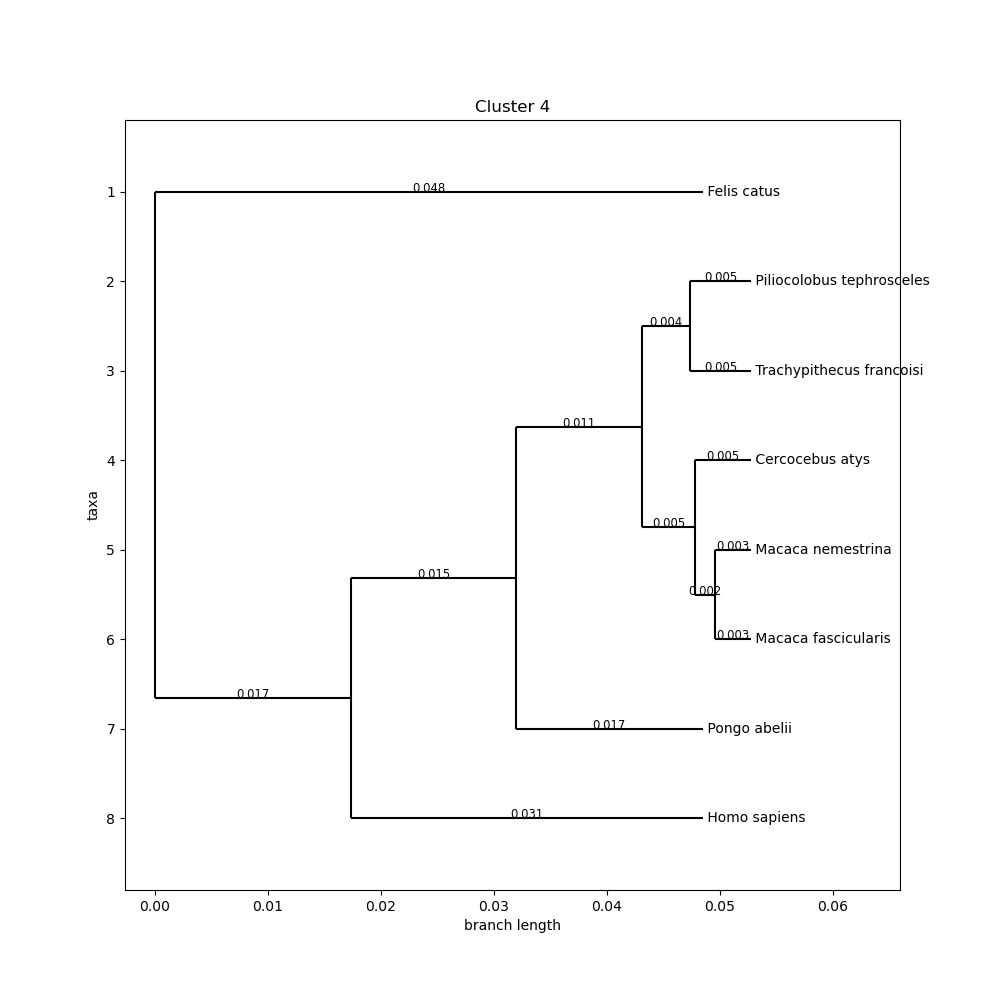
\includegraphics[width=0.45\textwidth]{Cluster 4.png} \\
        \hline
        \textit{Human leukocyte elastase (1PPF\_E)} & \textit{Cluster 4} \\
        \hline
        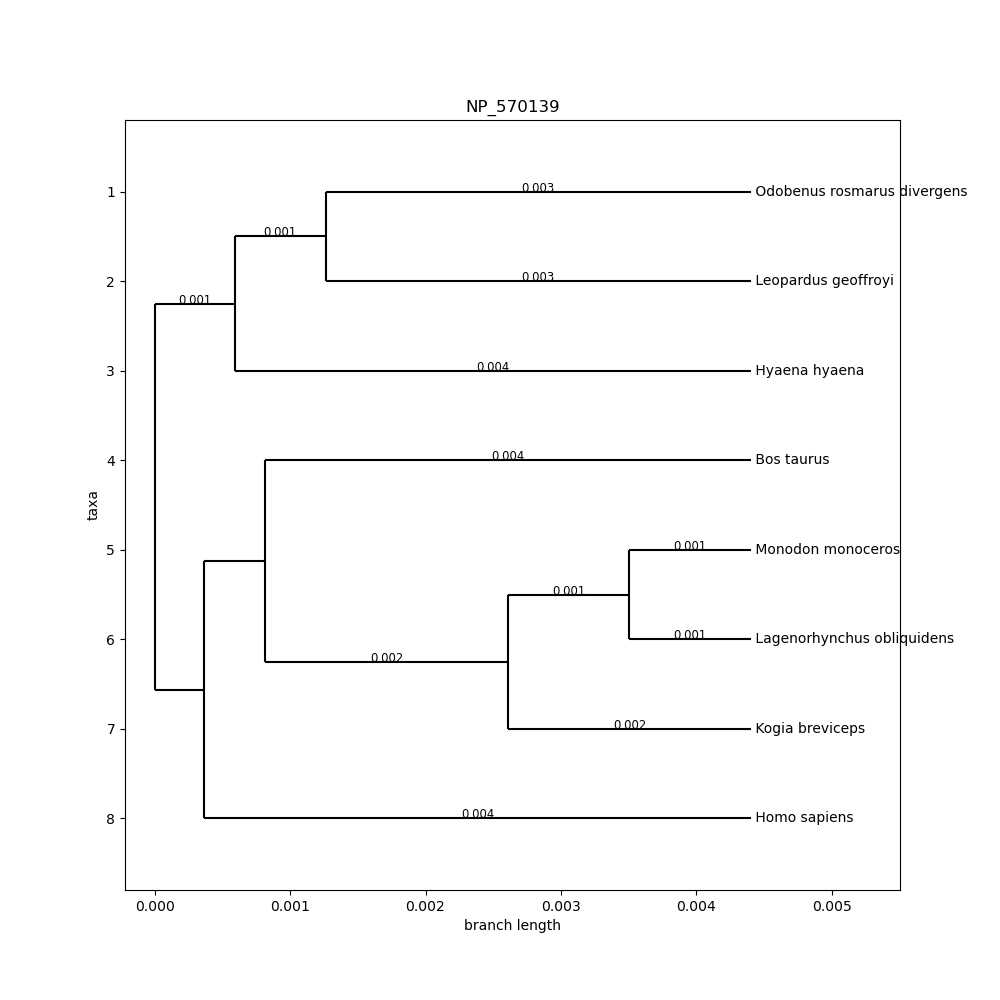
\includegraphics[width=0.45\textwidth]{NP_570139.png} &
        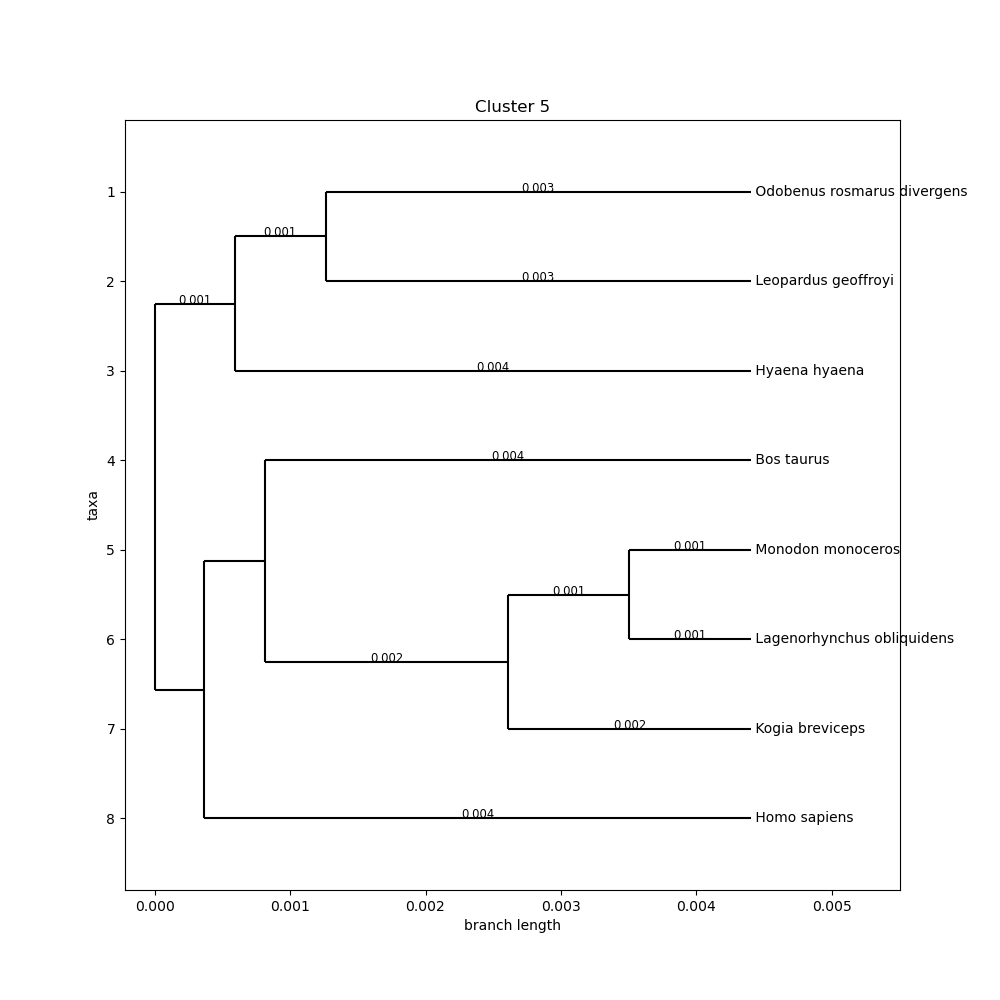
\includegraphics[width=0.45\textwidth]{Cluster 5.png} \\
        \hline
        \textit{Tetraspanin-18 (NP\_570139)} & \textit{Cluster 5} \\
        \hline
        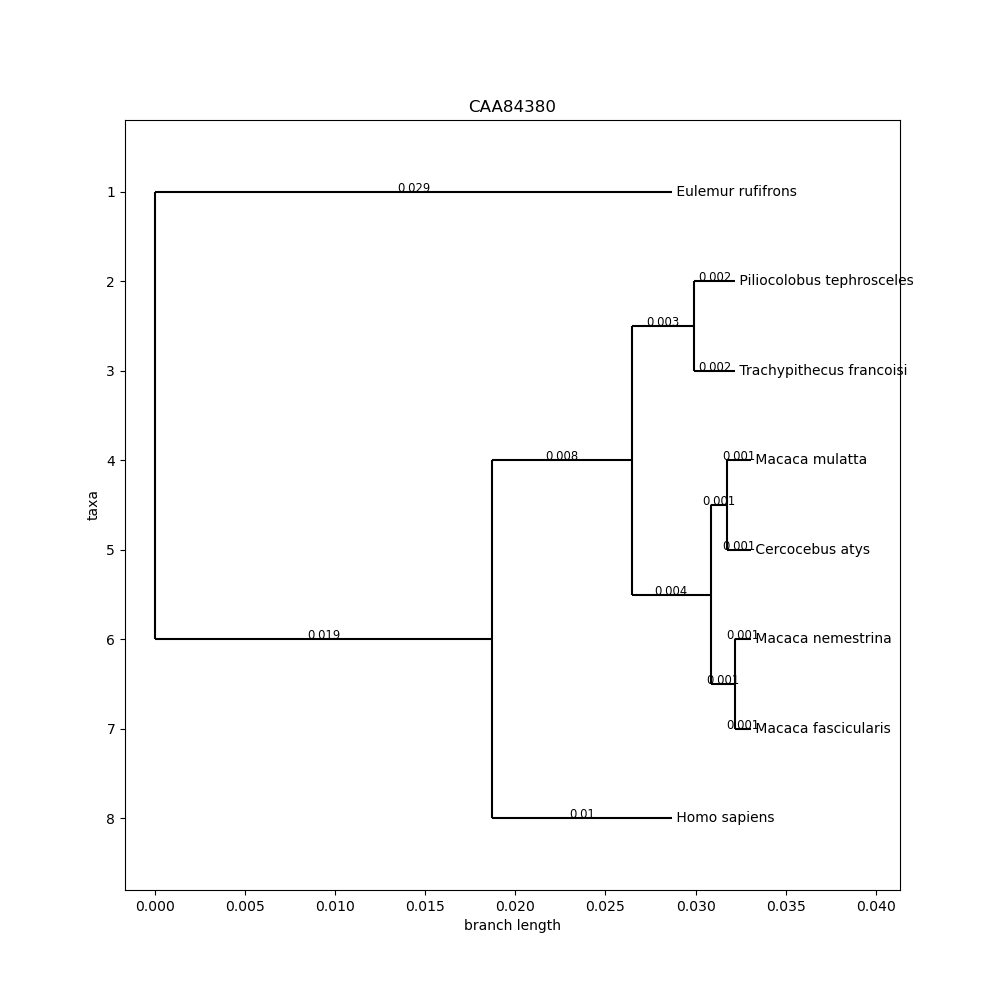
\includegraphics[width=0.45\textwidth]{CAA84380.png} &
        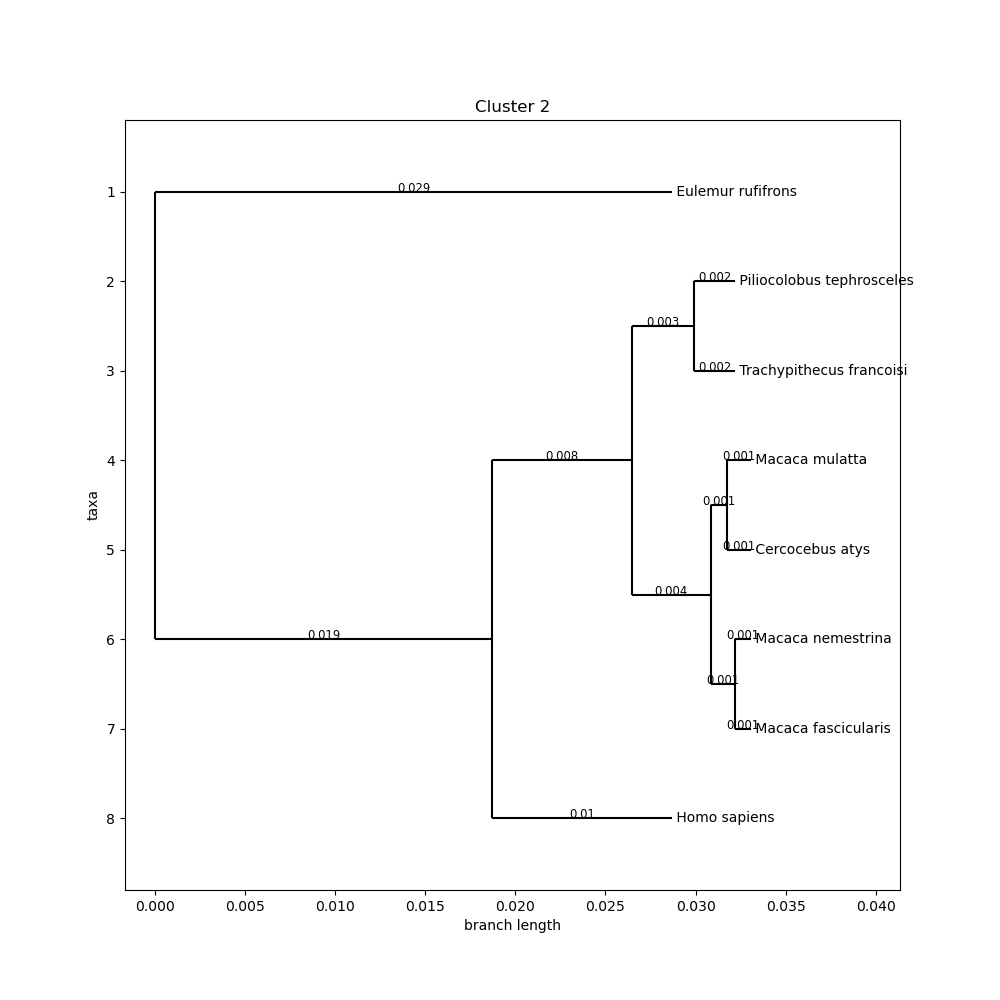
\includegraphics[width=0.45\textwidth]{Cluster 2.png} \\
        \hline
        \textit{Histamine H1 receptor (CAA84380)} & \textit{Cluster 2} \\
        \hline
        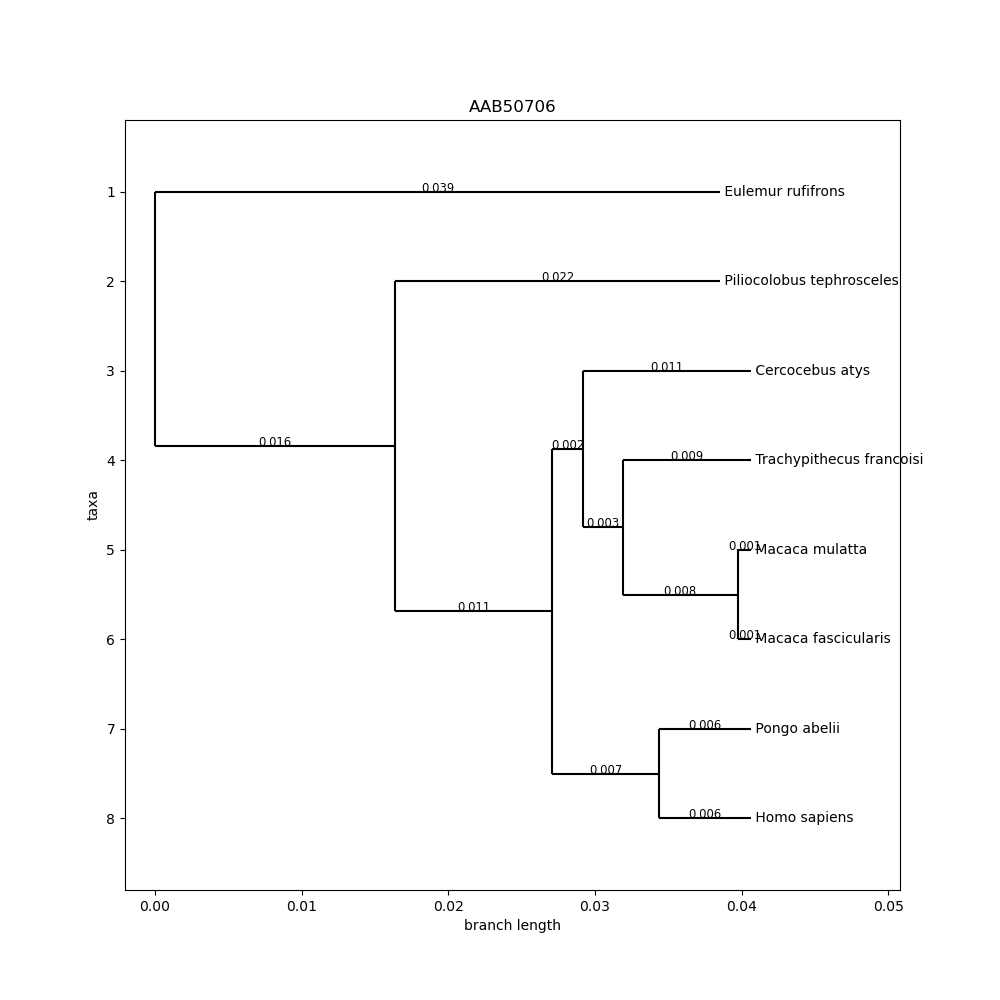
\includegraphics[width=0.45\textwidth]{AAB50706.png} &
        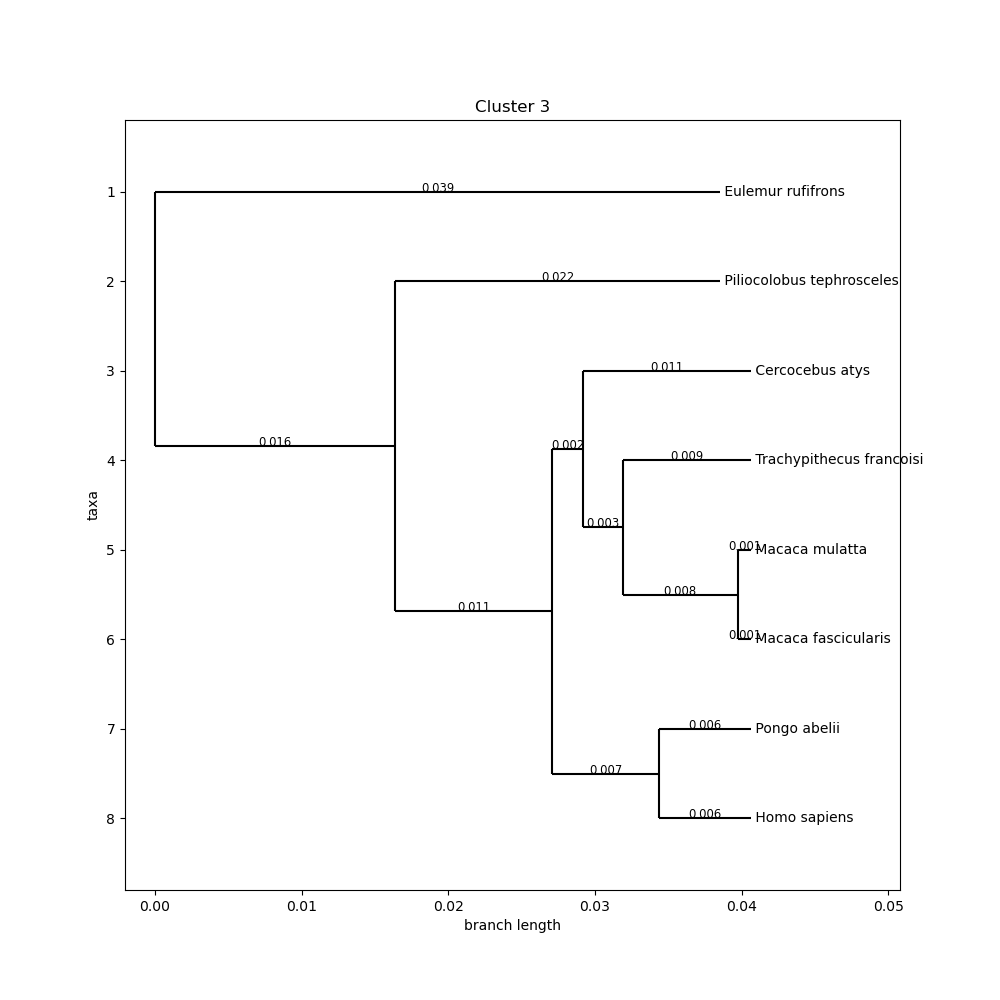
\includegraphics[width=0.45\textwidth]{Cluster 3.png} \\
        \hline
        \textit{Ficolin (AAB50706)} & \textit{Cluster 3} \\
        \hline
        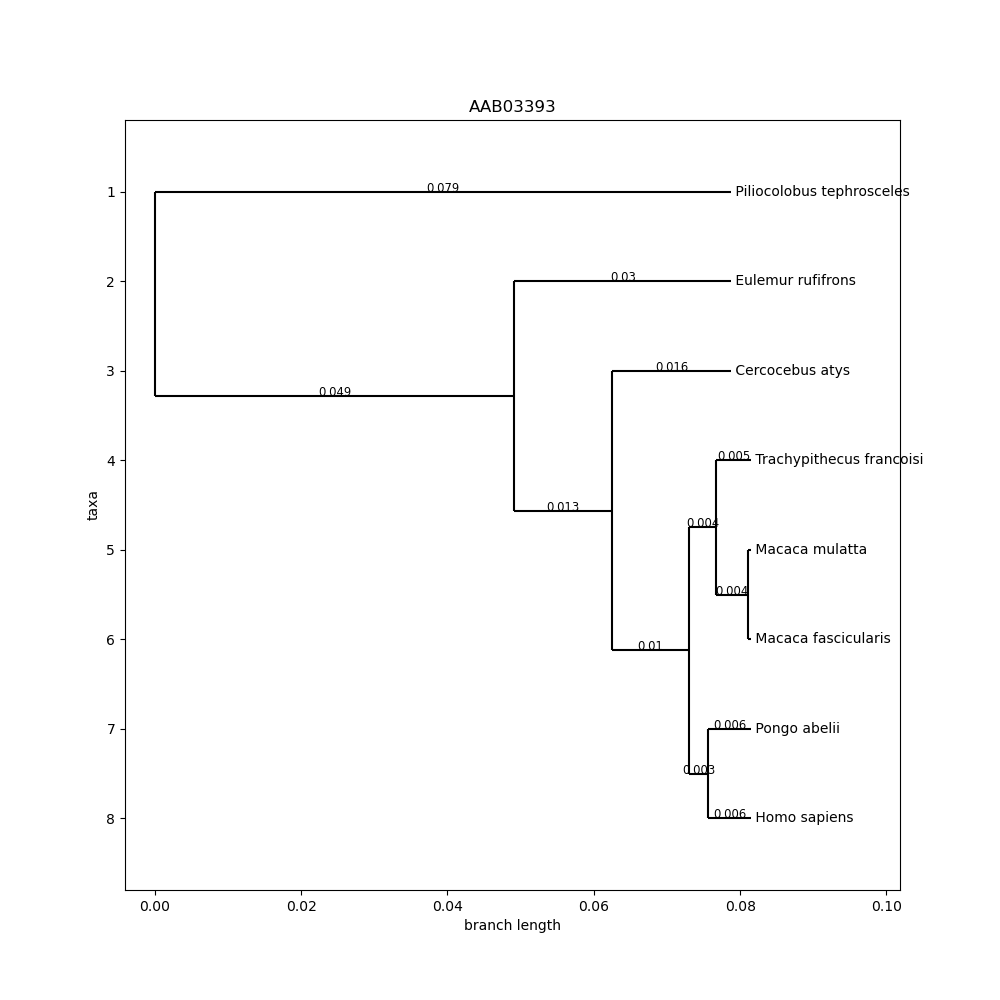
\includegraphics[width=0.45\textwidth]{AAB03393.png} &
        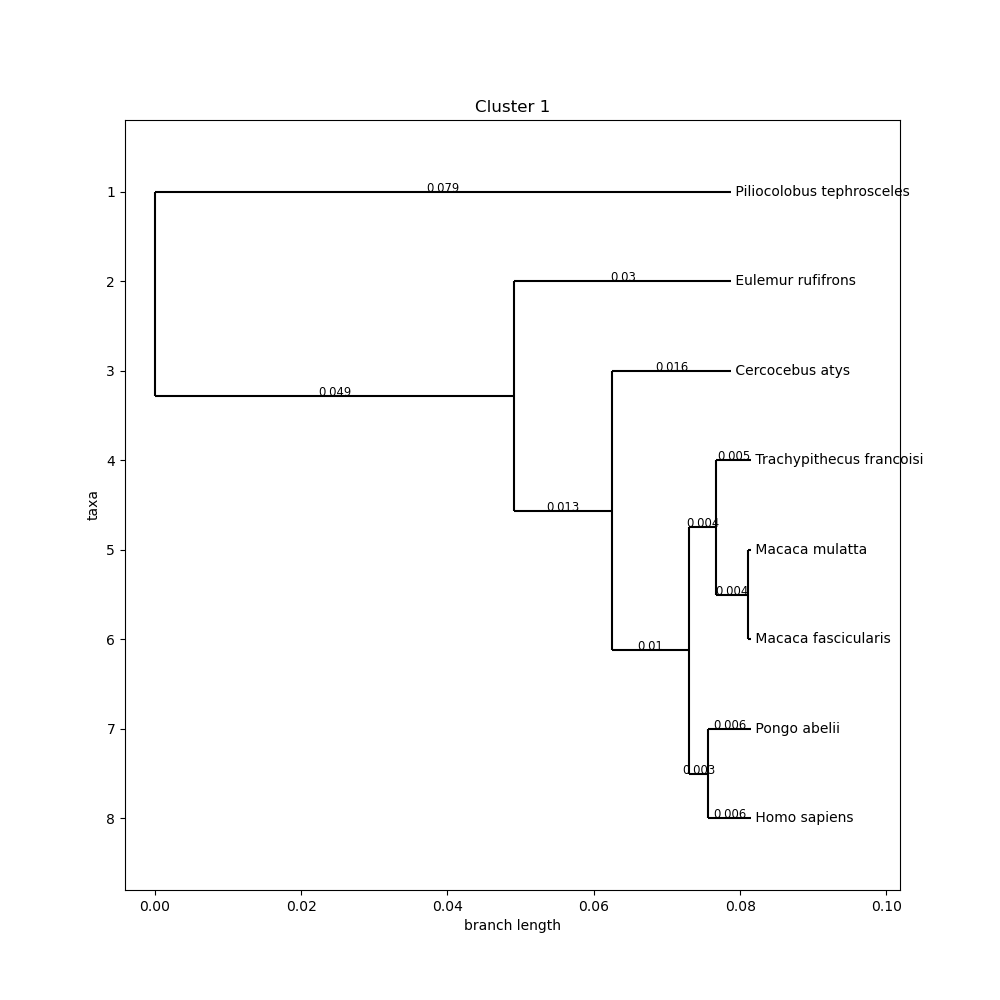
\includegraphics[width=0.45\textwidth]{Cluster 1.png} \\
        \hline
        \textit{Thrombopoietin (AAB03393)} & \textit{Cluster 1} \\
        \hline
        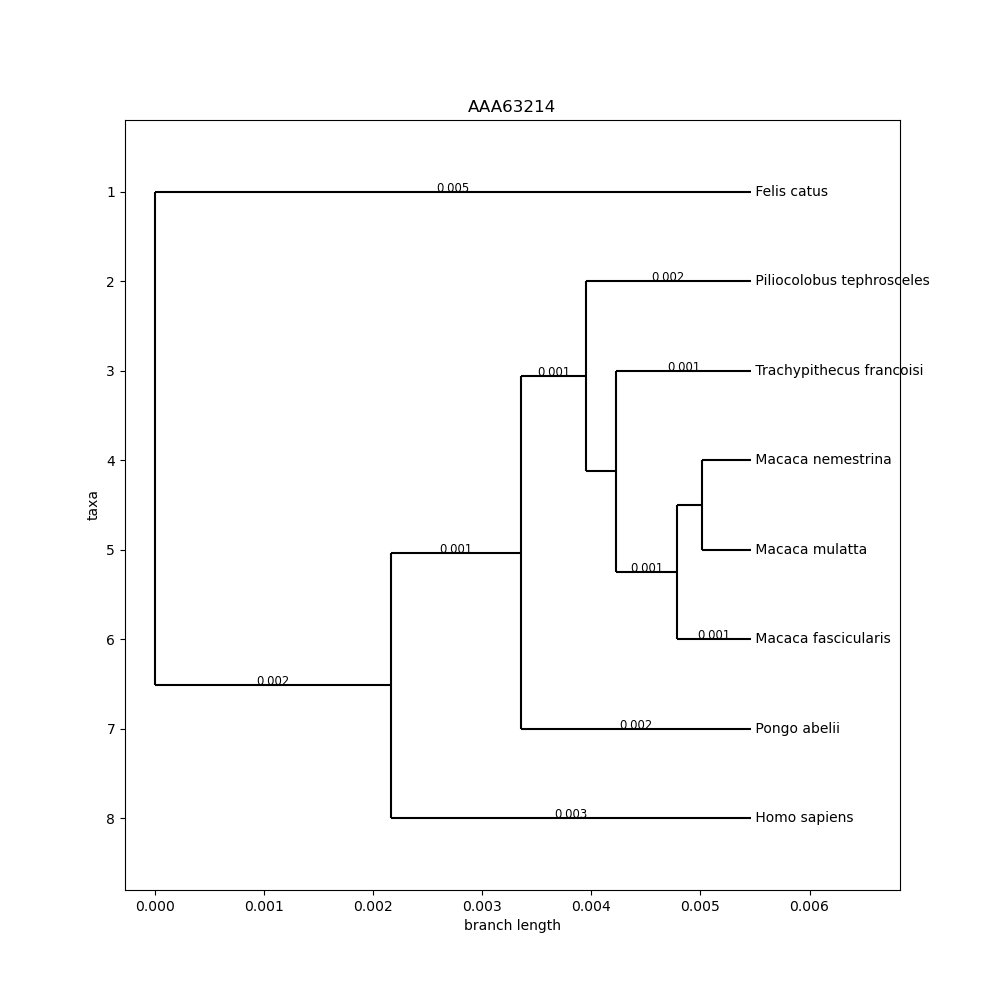
\includegraphics[width=0.45\textwidth]{AAA63214.png} &
        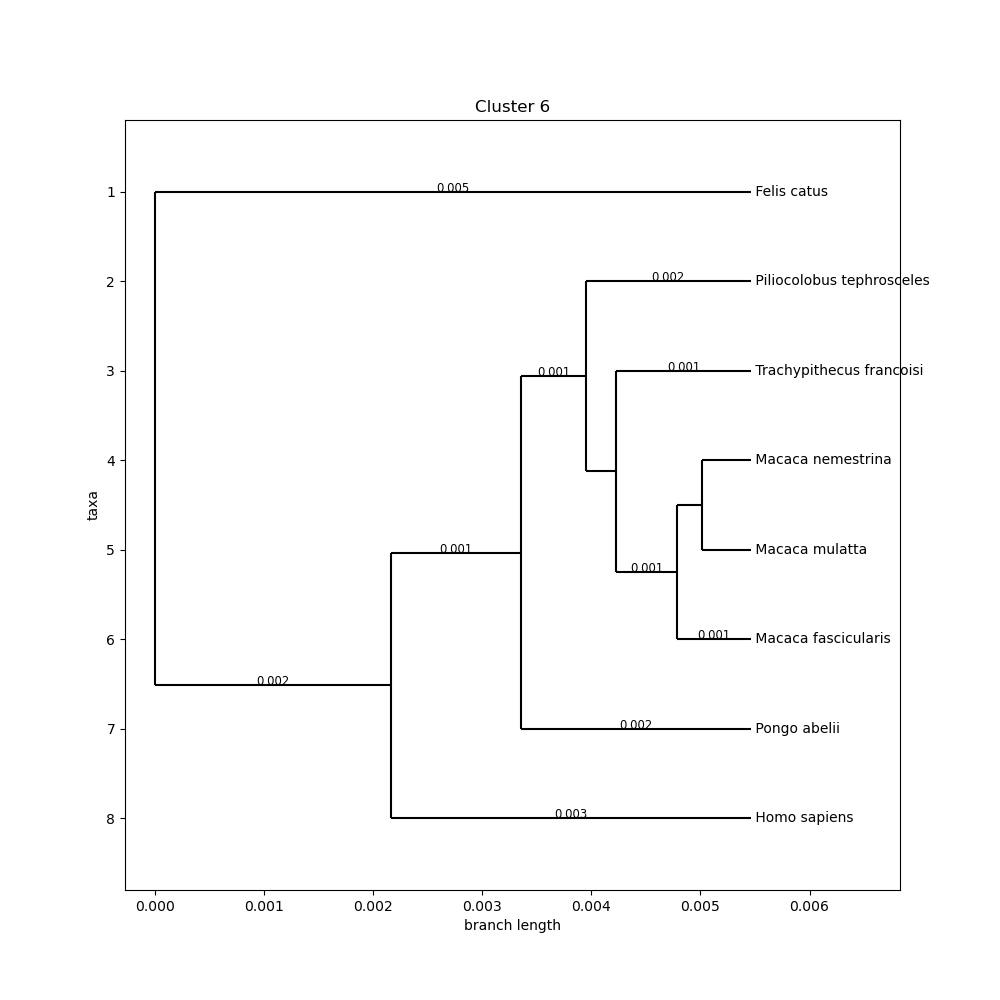
\includegraphics[width=0.45\textwidth]{Cluster 6.png} \\
        \hline
        \textit{Melanin concentrating hormone (AAA63214)} & \textit{Cluster 6} \\
        \hline
        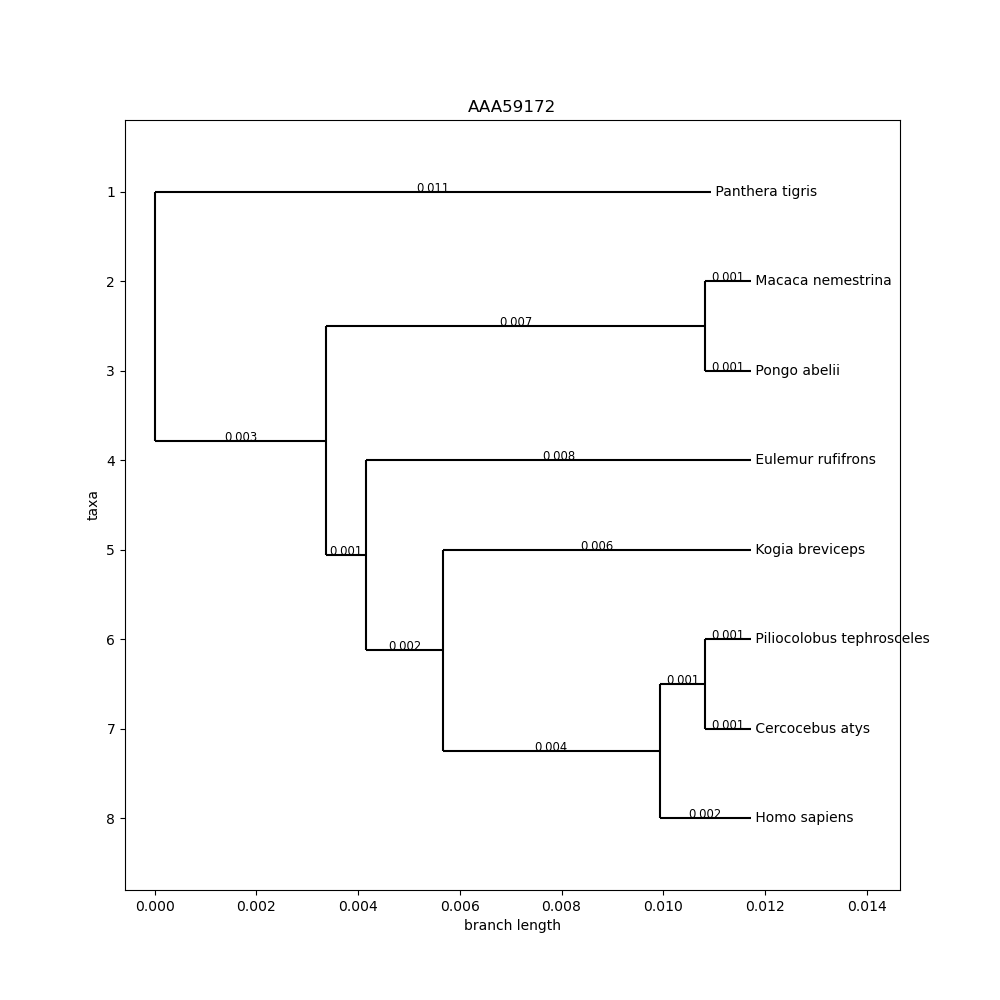
\includegraphics[width=0.45\textwidth]{AAA59172.png} &
        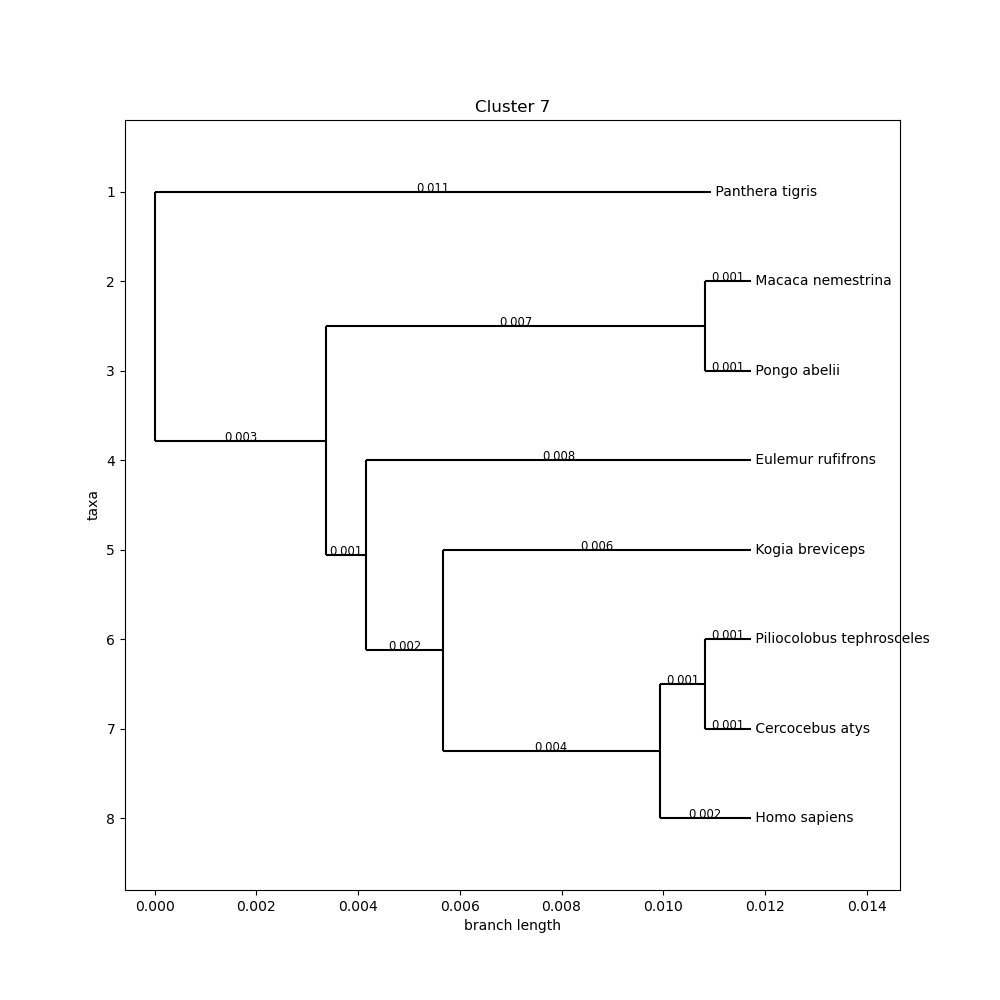
\includegraphics[width=0.45\textwidth]{Cluster 7.png} \\
        \hline
        \textit{Insulin (AAA59172)} & \textit{Cluster 7} \\
        \hline
        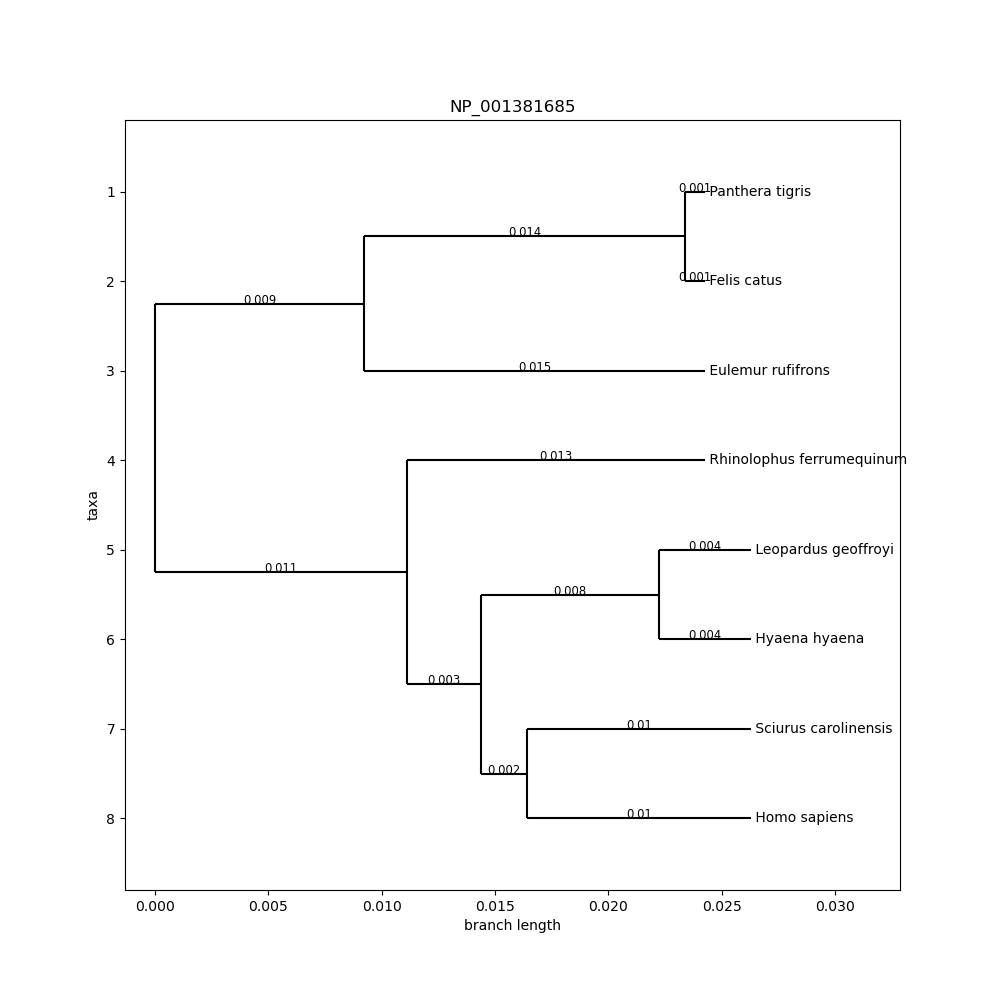
\includegraphics[width=0.45\textwidth]{NP_001381685.png} &
        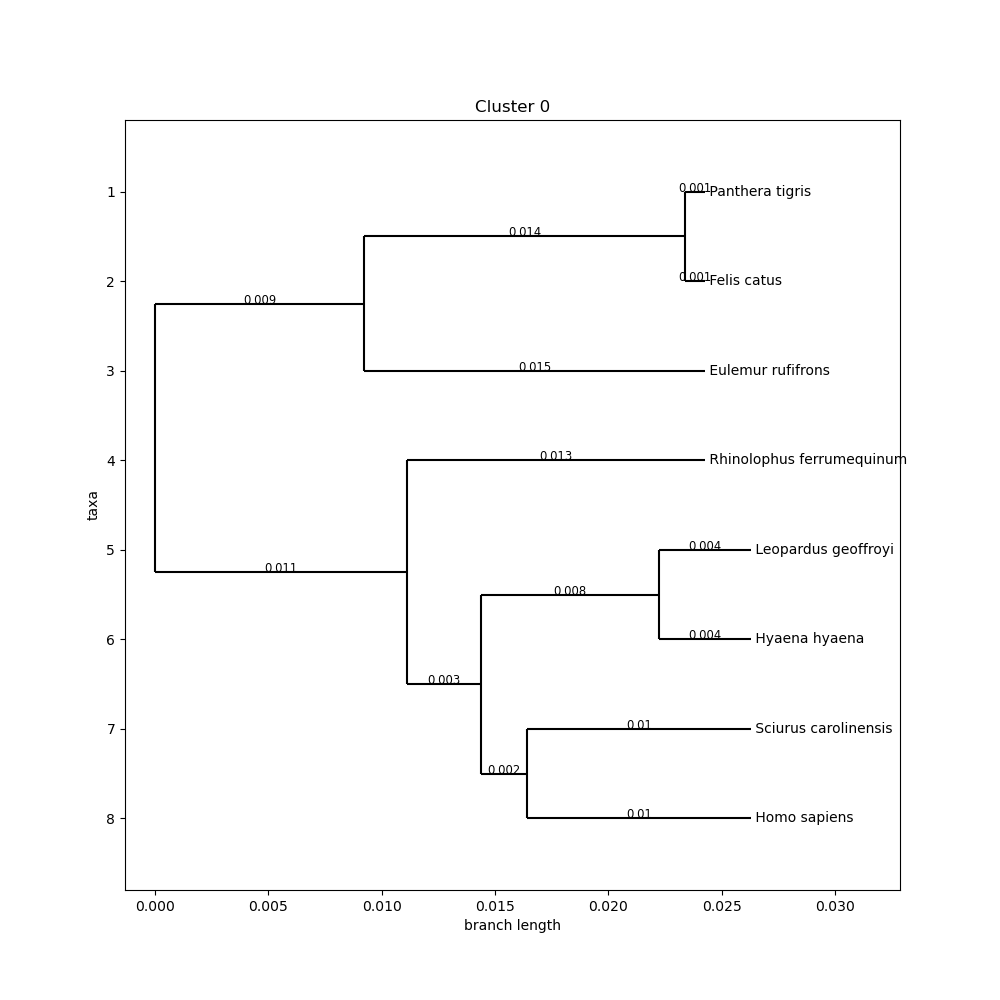
\includegraphics[width=0.45\textwidth]{Cluster 0.png} \\
        \hline
        \textit{TANK-binding kinase 1-binding protein 1 (NP\_001381685)} & \textit{Cluster 0} \\
        \hline
%    \end{tabular}
    \caption{Comparison between original protein trees and their corresponding cluster trees. The matching topology and branch lengths across all pairs demonstrate the consistency of the clustering approach with the original protein groupings.}
    \label{fig:tree_pairs}
\end{longtable}

The comparison reveals perfect correspondence between the trees generated from original protein groups and their matching clusters. This remarkable similarity extends across all eight protein families, with identical topological structures and highly similar branch lengths. This correspondence validates both our initial protein selection and the effectiveness of the CD-HIT clustering algorithm in identifying natural protein families.

\subsection{Consensus Trees Analysis}\label{subsec:consensus-trees-analysis}

The consensus trees generated from both approaches - protein groups and clusters - provide insights into the overall evolutionary relationships between the studied organisms. Figure~\ref{fig:consensus_trees} shows both consensus trees colored by organism for direct comparison.

\begin{figure}[H]
    \centering
    \begin{tabular}{cc}
        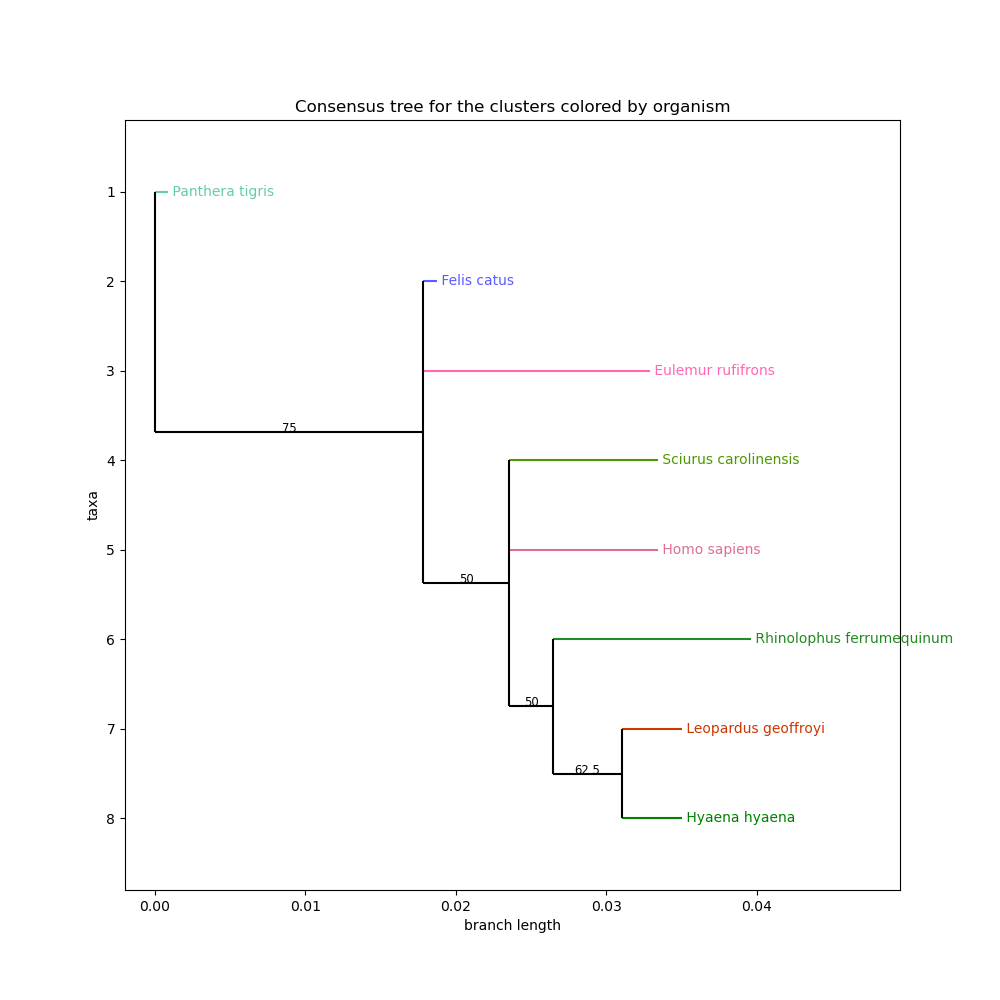
\includegraphics[width=0.45\textwidth]{clusters_consensus_colored.png} &
        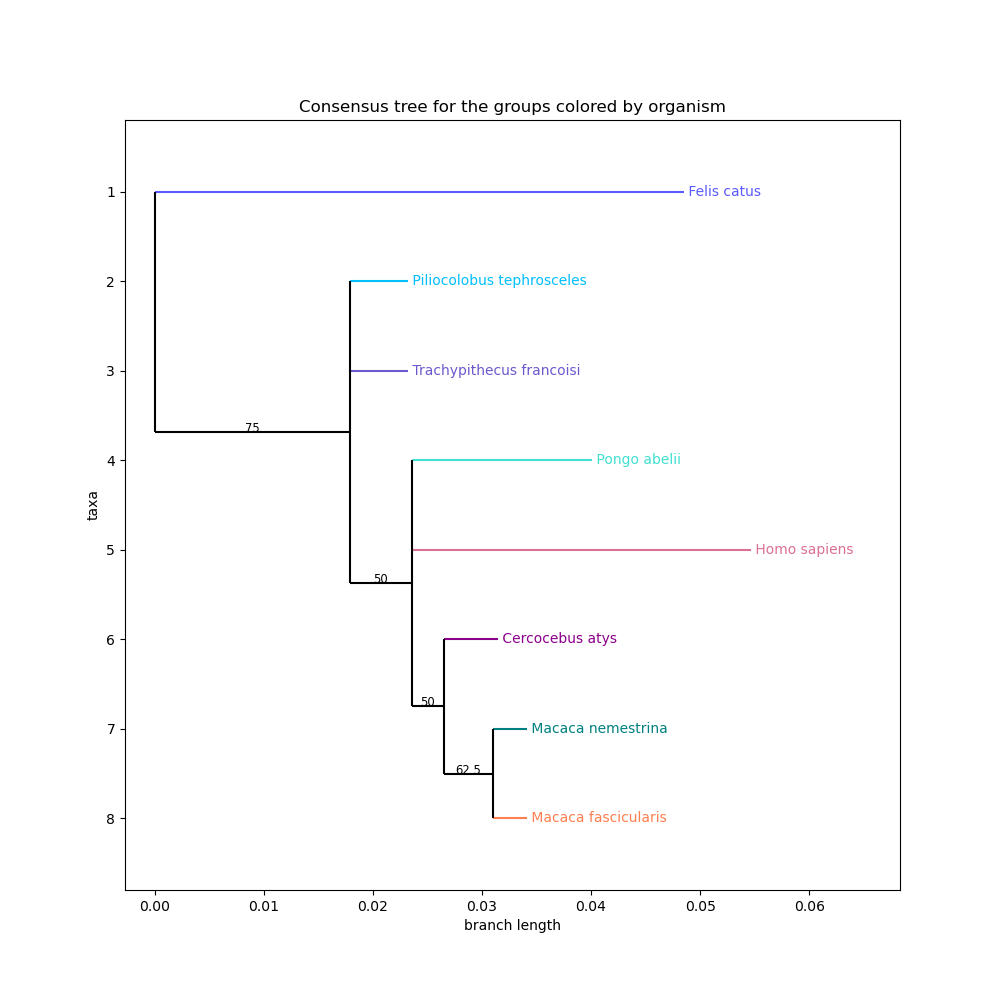
\includegraphics[width=0.45\textwidth]{groups_consensus_colored.png} \\
        (a) Cluster-based consensus tree & (b) Protein group-based consensus tree
    \end{tabular}
    \caption{Consensus trees from cluster-based and protein group-based analyses, colored by organism. Numbers at internal nodes represent the percentage of trees supporting each split.}
    \label{fig:consensus_trees}
\end{figure}

Several key observations can be made from comparing these consensus trees:

\begin{enumerate}
    \item \textbf{Topology Similarities:}
    \begin{itemize}
        \item Both trees show similar major groupings with primates clustering together
        \item Human (Homo sapiens) and orangutan (Pongo abelii) maintain their close evolutionary relationship
    \end{itemize}

    \item \textbf{Notable Differences:}
    \begin{itemize}
        \item The cluster consensus tree includes additional species like Panthera tigris and Sciurus carolinensis that appear in some but not all protein groups
        \item Branch support values (shown as percentages at nodes) differ between the trees, suggesting varying levels of confidence in different evolutionary relationships
    \end{itemize}

    \item \textbf{Evolutionary Implications:}
    \begin{itemize}
        \item Support values of 75\% at the deepest nodes suggest strong confidence in the major evolutionary divisions
        \item Lower support values (50-62.5\%) at some internal nodes indicate areas where evolutionary relationships are less certain
    \end{itemize}
\end{enumerate}

The differences between the two consensus trees can be attributed to several factors:

\begin{enumerate}
    \item The CD-HIT clustering threshold (50\%) may group sequences slightly differently than the initial protein-based selection, particularly for more divergent homologs.
    \item Consensus trees are based on the majority rule, which can lead to differences in branch support values depending on the number of trees supporting a particular split.
    \item The algorithm behind may be non-deterministic, leading to slight variations in the consensus tree topology. Having more data (more sequences, more proteins) would likely increase the robustness of the consensus tree.
\end{enumerate}

\subsection{Full Tree Analysis with Different Coloring Schemes}\label{subsec:full-tree-analysis-with-different-coloring-schemes}

The full phylogenetic tree containing all sequences was visualized using two different coloring schemes to highlight different aspects of evolutionary relationships. Figure~\ref{fig:full_trees} shows the complete tree colored by protein group and by organism.

\begin{figure}[H]
    \centering
    \begin{tabular}{cc}
        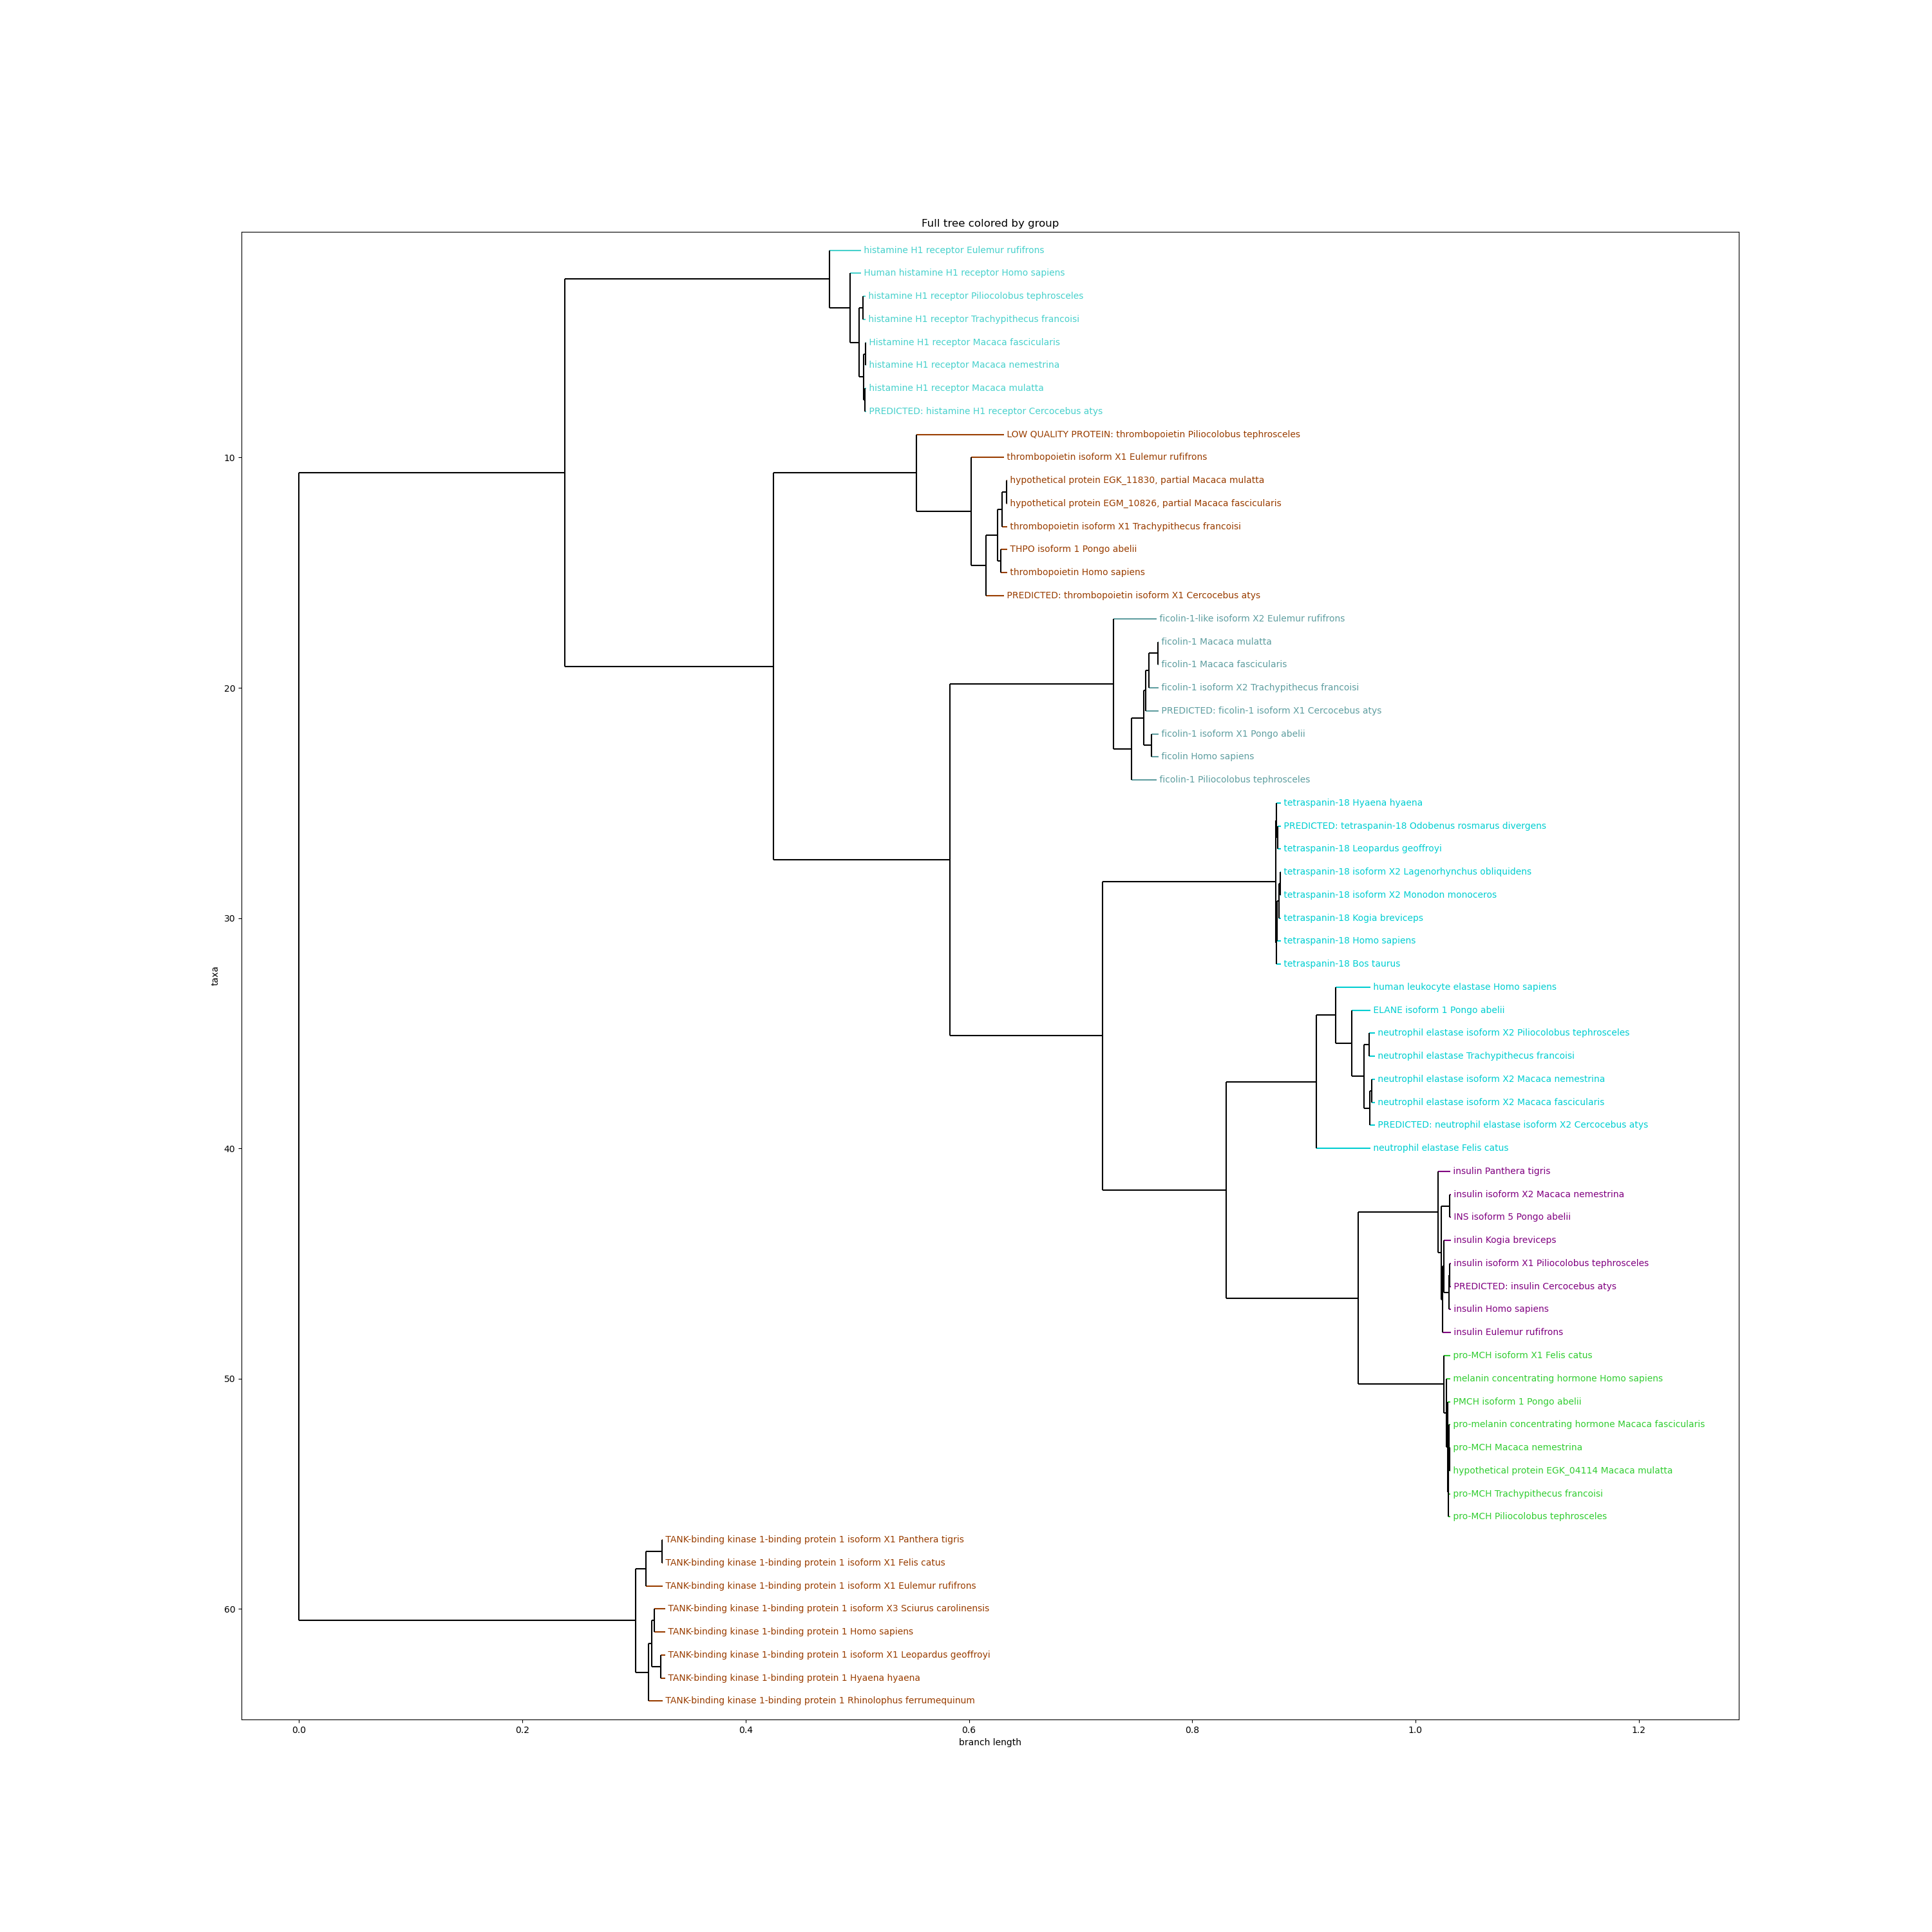
\includegraphics[width=0.45\textwidth]{full_colored_by_group.png} &
        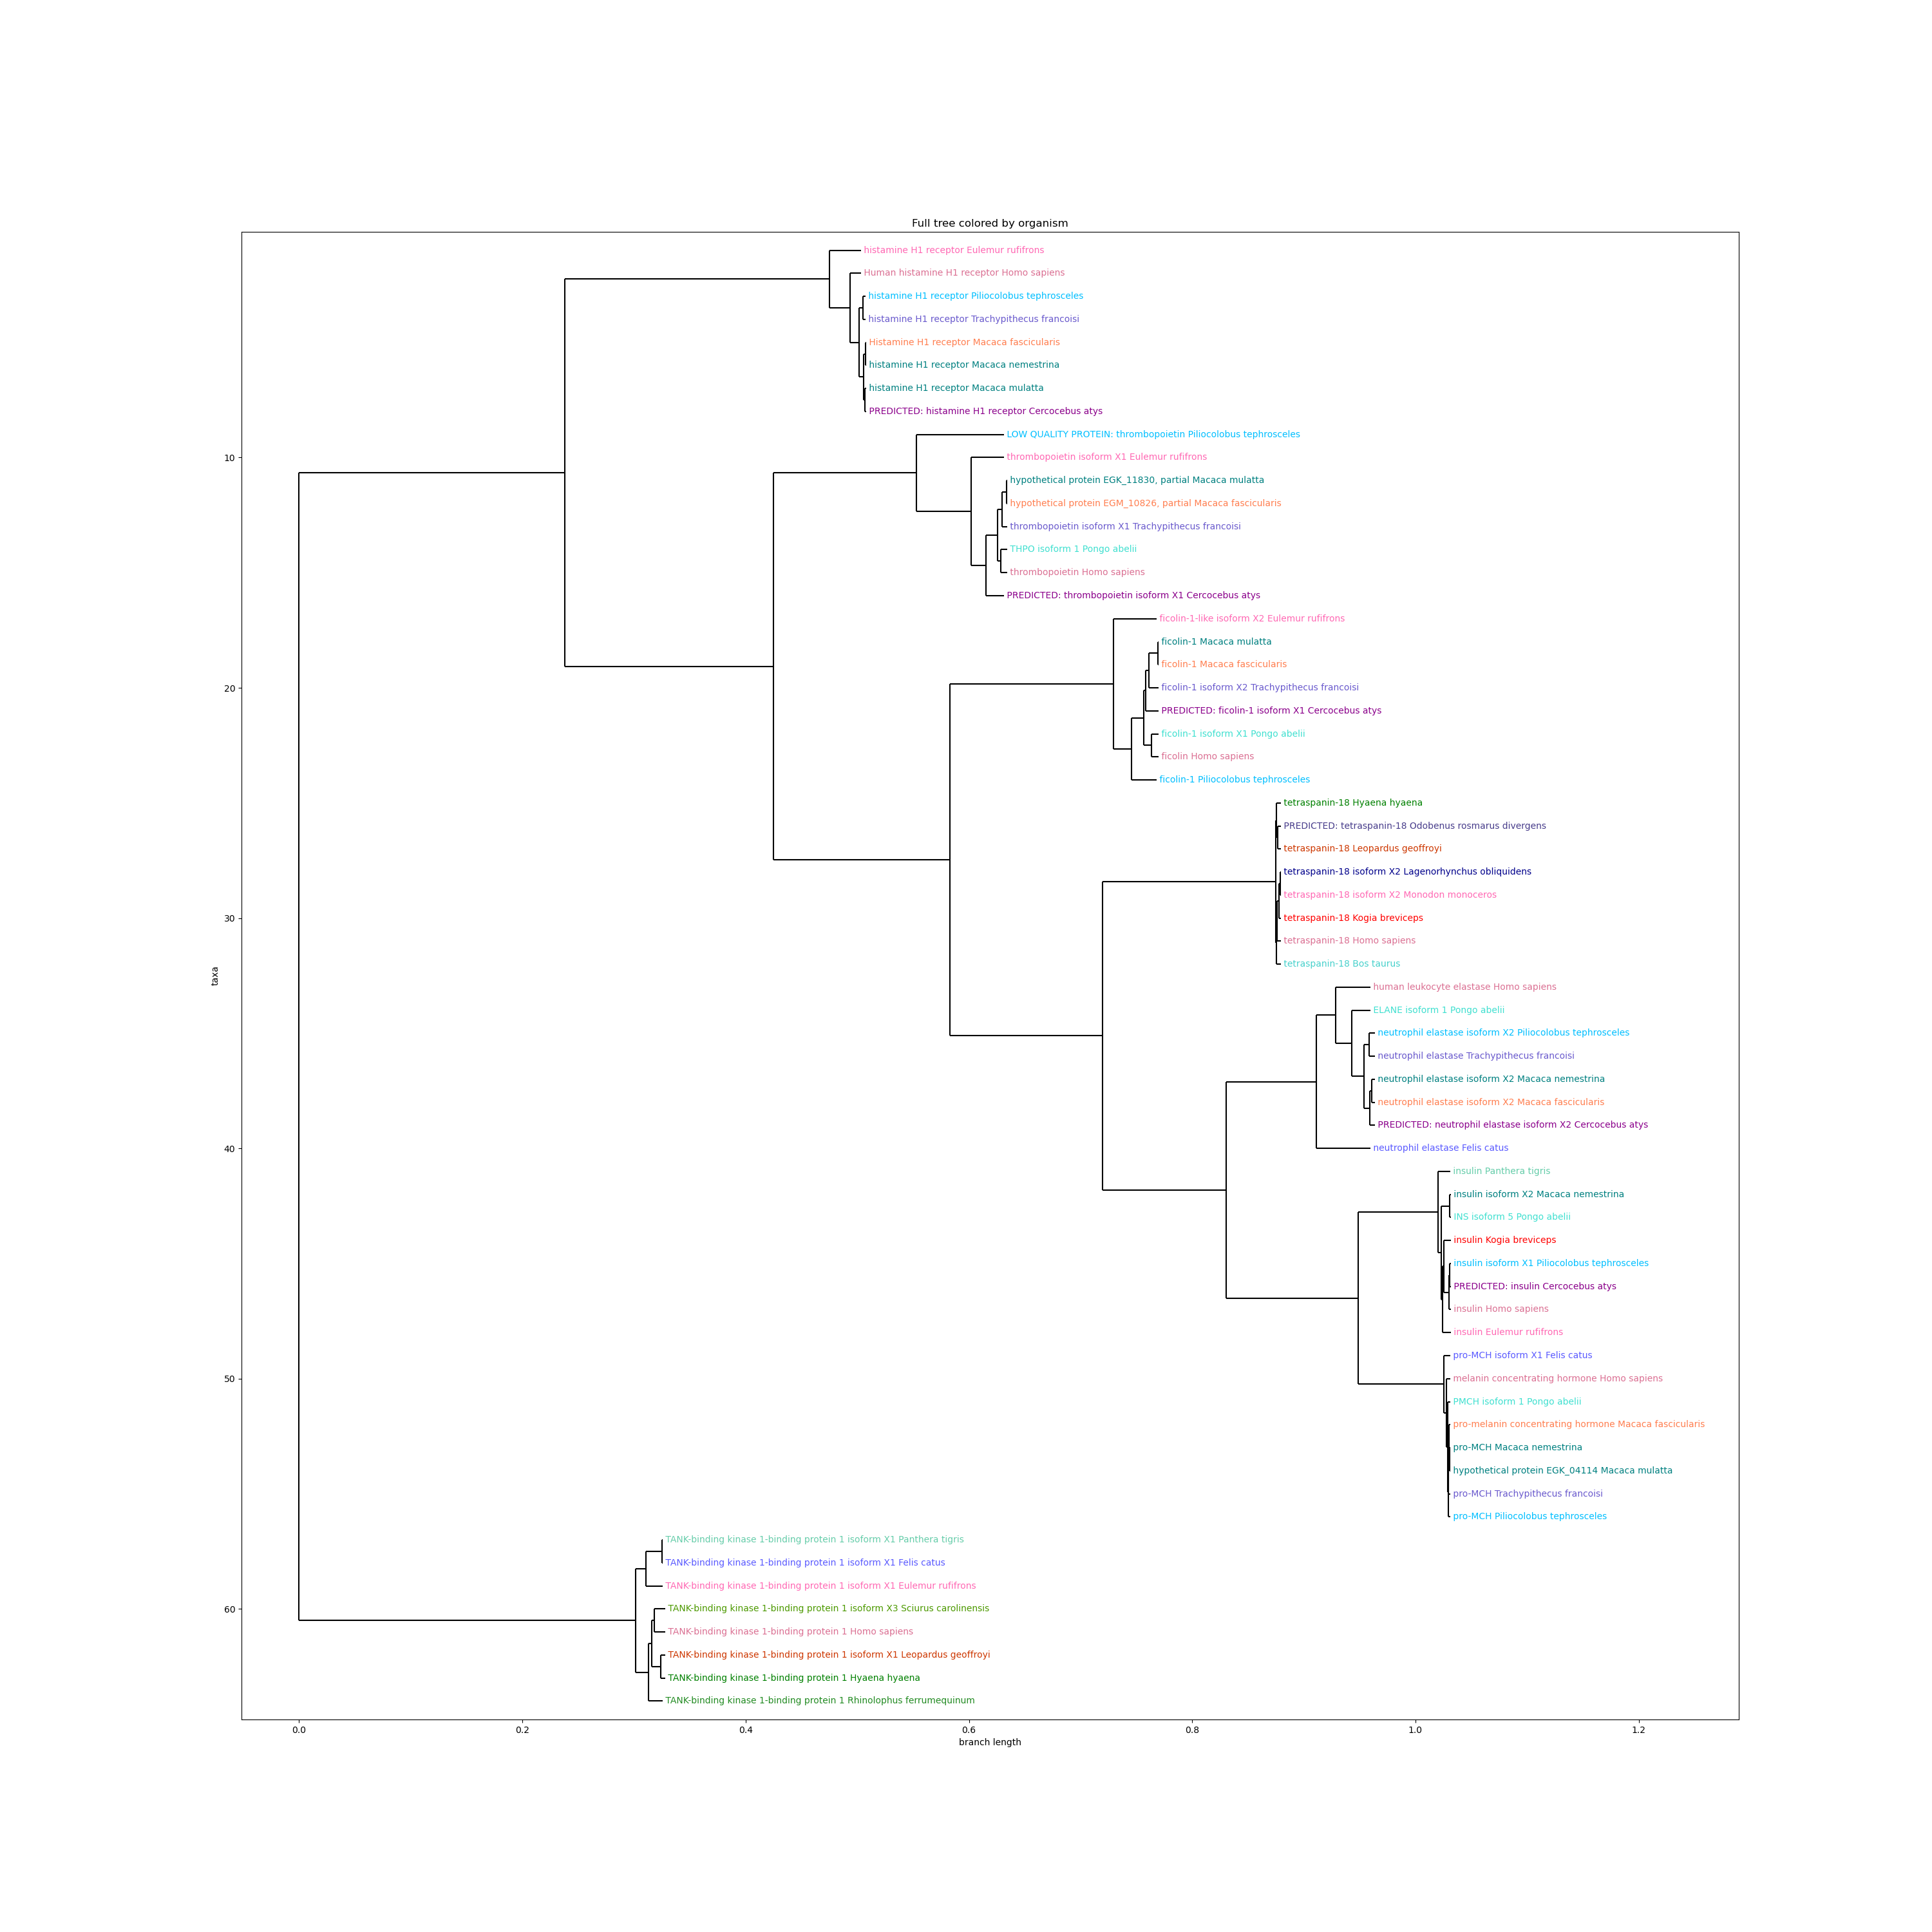
\includegraphics[width=0.45\textwidth]{full_colored.png} \\
        (a) Colored by protein group & (b) Colored by organism
    \end{tabular}
    \caption{Full phylogenetic tree visualized with different coloring schemes. (a) Colors represent different protein families, showing functional grouping. (b) Colors represent different organisms, highlighting species relationships.}
    \label{fig:full_trees}
\end{figure}

The two coloring schemes reveal different aspects of the evolutionary relationships:

\begin{enumerate}
    \item \textbf{Protein-based Coloring (a):}
    \begin{itemize}
        \item Clearly shows the clustering of protein families, with each color representing a distinct functional group
        \item Demonstrates that sequence similarity is primarily driven by protein function rather than species relationships
        \item Reveals deep evolutionary divergence between different protein families (long branches between different colors)
        \item Shows conservation of protein function across species (same-colored clusters containing different organisms)
    \end{itemize}

    \item \textbf{Organism-based Coloring (b):}
    \begin{itemize}
        \item Highlights the distribution of species across different protein families
        \item Shows that sequences from the same organism can be found in different parts of the tree
        \item Demonstrates that evolutionary rates vary among different proteins within the same species
        \item Reveals patterns of species-specific variation within protein families
    \end{itemize}
\end{enumerate}

Key observations from comparing both colorings:
\begin{itemize}
    \item The deepest branches in the tree separate different protein families rather than different organisms
    \item Within each protein family cluster, sequences generally group by species relatedness
    \item The TANK-binding kinase 1-binding protein 1 family (bottom cluster) shows the most distinct separation from other proteins
    \item Some proteins show more species-specific variation than others, as indicated by the distribution of organism colors within protein groups
\end{itemize}

\subsection{Answers to the questions}\label{subsec:answers-to-the-questions}

\paragraph{d) Observations and Best Approach}

After analyzing the different approaches to tree construction and visualization, several key observations can be made:

\paragraph{Tree Construction Approaches:}
\begin{itemize}
    \item Consensus trees provide a summarized view of evolutionary relationships but may lose some detail
    \item The single tree from all sequences offers a more comprehensive view of evolutionary relationships across all proteins and species
    \item The single tree approach better preserves the complexity of evolutionary relationships, showing both protein-specific and species-specific patterns
\end{itemize}

\paragraph{Coloring Approaches:}
\begin{itemize}
    \item Organism-based coloring highlights:
    \begin{itemize}
        \item Species distribution across different protein families
        \item Consistency of evolutionary relationships within species
        \item Variable evolutionary rates among species
    \end{itemize}
    \item Protein group-based coloring reveals:
    \begin{itemize}
        \item Clear separation between protein families
        \item Functional clustering of sequences
        \item Conservation of protein functions across species
    \end{itemize}
\end{itemize}

The single tree with dual coloring schemes appears to work best for this analysis because:
\begin{itemize}
    \item It provides the most comprehensive view of both protein and species evolution
    \item Different coloring schemes complement each other, revealing different aspects of evolution
    \item It maintains all evolutionary information without the averaging effect seen in consensus trees
    \item It allows direct comparison of evolutionary patterns between different protein families
\end{itemize}

\paragraph{e) Tree Similarity and Evolutionary Patterns}

When comparing the different trees, we observe both similarities and differences:

1. \textbf{Similarities:}
\begin{itemize}
    \item Major evolutionary relationships are conserved across all approaches
    \item Primate species consistently cluster together
    \item Branch lengths within protein families are comparable
    \item The relative positions of closely related species (e.g., Macaca species) remain stable
\end{itemize}

2. \textbf{Differences:}
\begin{itemize}
    \item The cluster-based approach includes some additional species relationships, while excluding others
    \item Support values for some internal nodes differ between approaches
    \item The full tree shows more complex patterns than individual protein trees
    \item Some species show different positions depending on the protein family being analyzed
\end{itemize}

The evolution does not look exactly the same in different trees because:
\begin{itemize}
    \item Different proteins evolve at different rates
    \item Some proteins may be under different selective pressures in different species
    \item The clustering approach may capture different aspects of sequence similarity
    \item The consensus trees represent a "democratic average" of multiple evolutionary histories
\end{itemize}

\end{document}